\documentclass{ximera}

\begin{document}

\begin{question}
  Find 
  \[
  \displaystyle \lim_{x\to 0} x^3-3x^2+x-5
  \]
  \begin{solution}
    \begin{hint}
      This function is continuous everywhere. Therefore, left-hand and right-hand limits exist at every point and are equal. Use this to your advantage.
    \end{hint}
     \begin{hint}
    Take a look at the graph of the function
    \begin{center}
     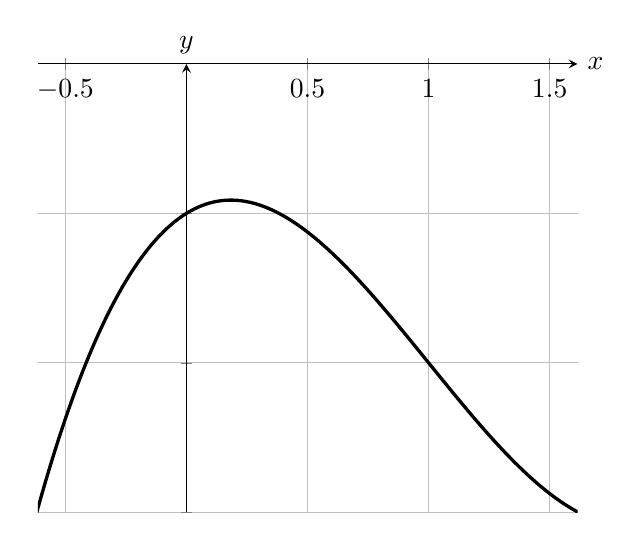
\begin{tikzpicture}
	\begin{axis}
	[ymin=-7,ymax=-4, axis lines=center,xlabel=$x$,ylabel=$y$,every axis y 
	label/.style={at=(current axis.above origin),anchor=south},every axis x label/.style={at=(current axis.right of origin),anchor=west},
	domain=-2:2,
	yticklabels={},
	ymajorgrids=true,
	grid = major
	]
	\addplot[very thick,smooth,samples=500]
	{\x^3-3*\x^2+\x-5};
	\end{axis}
       \end{tikzpicture}      
      \end{center}
    \end{hint}
    \begin{hint}
     Evaluating $\left.x^3-3x^2+x-5\right|_{x=0}$ gives $-5$. This seems reasonable because there are no discontinuities in $x^3-3x^2+x-5$.
    \end{hint}
    $\displaystyle{\lim_{x\to0}x^3-3x^2+x-5}=$
    \answer{$-5$}.
  \end{solution}
\end{question}

\end{document}